\documentclass[letter]{article}
\renewcommand{\baselinestretch}{1.25}

\usepackage[margin=1in]{geometry}
\usepackage{physics}
\usepackage{amsmath, mathtools}
\numberwithin{equation}{section}
\usepackage{amssymb}
\usepackage{graphicx}
\usepackage{hyperref}
\usepackage{empheq}

% MATLAB Formating Code
\usepackage[numbered,framed]{matlab-prettifier}
\lstset{style=Matlab-editor,columns=fullflexible}
\renewcommand{\lstlistingname}{Script}
\newcommand{\scriptname}{\lstlistingname}

% Document Specific
\newcommand{\sat}{\text{sat}}
\newcommand{\sign}{\text{sign}}

\allowdisplaybreaks

%opening
\title{MECH 6313 - Term Exam}
\author{\textbf{Name:} Jonas Wagner\\ \textbf{UTD ID:} 2021531784}
\date{2021, April 30}

\begin{document}

\maketitle

\tableofcontents

%----------------------------------------------------------------------------
\newpage
\section{Problem 1}
Consider the system:
\begin{equation}
	\begin{aligned}
		\tau \dot{x} &= x - \frac{1}{3} x^3 - y\\
		\dot{y} &= x + \mu
	\end{aligned}
\end{equation}
where $\tau > 0$ and $\mu \geq 0$ are constants.

\subsection{Part a}
\textbf{Problem:}
Determine the equilibrium points and classify their stability properties depending on the values of parameter $\mu$.\\

\noindent
\textbf{Solution:}
\subsubsection{Equilibrium Point Identification}
The equilibrium points exist whenever $\dot{x} = \dot{y} = 0$ and can be identified as follows:
\begin{align}
	&\begin{aligned}
		\tau \qty(0) &= x - \frac{1}{3} x^3 - y\\
		\qty(0) &= x + \mu
	\end{aligned}\\
\intertext{which becomes:}
	&\begin{aligned}
		y &= x - \frac{1}{3} x^3\\
		x &= -\mu
	\end{aligned}\\
\intertext{and can then substituted in as:}
	&\begin{aligned}
		x_{eq} &= -\mu\\
		y_{eq} &= -\mu - \frac{1}{3} (-\mu)^3
	\end{aligned}
\end{align}
This results in the equilibrium points being defined in terms of $\mu$ as:
\begin{empheq}[innerbox = \fbox]{equation}
	\begin{aligned}
		x_{eq} &= -\mu\\
		y_{eq} &= \frac{1}{3} \mu^3 - \mu
	\end{aligned}
\end{empheq}

\newpage
\subsubsection{System Linearization}
The stability around an equilibrium point can be evaluated by looking at the linearized model, which can be found as follows:\\

Let the state-variables be defined as:
$$X = \mqty[x\\ y]$$
The nonlinear state equation would then be defined as:
\begin{equation}
	\dot{X} = f(x) 
	= \mqty[\cfrac{x_1 - \frac{1}{3} x_1^3 - x_2}{\tau}\\
			x_1 + \mu]
\end{equation}

Then the equilibrium point is described as
$$X_{eq} = \mqty[-\mu\\ \frac{1}{3} \mu^3 - \mu]$$
and the jacobian can be computed as:
\begin{align}
	J_x = \dv{f}{X} &= \mqty[\dv{f_1}{x_1} &\dv{f_1}{x_2}\\ \dv{f_2}{x_1} & \dv{f_2}{x_2}]\\
	&= \mqty[\cfrac{1 - x_1^2}{\tau} & -1\\
			 1 & 0]
\end{align}

The state dynamics around the equilibrium are described by this Jacobian evaluated at $X = X_{eq}$:
\begin{align}
	A = \eval{J_x}_{X = X_{eq}}
	&= \eval{\mqty[\cfrac{1 - x_1^2}{\tau} & -1\\ 1 & 0]}_{x_1 = -\mu, x_2 = \frac{1}{3} \mu^3 - \mu}\\
	&= \mqty[\cfrac{1 - (-\mu)^2}{\tau} & -1\\ 1 & 0]\\
	&= \mqty[\frac{1}{\tau} - \frac{\mu^2}{\tau} &-1\\ 1 &0]
\end{align}

The dynamics of this linearized system are described by the characteristic polynomial calculated as:
\begin{align}
	\Delta(s) = \det(sI - A)
	&= \det\mqty[s-\qty(\frac{1}{\tau} - \frac{\mu^2}{\tau}) &1\\ -1 &s]\\
	&= s \qty(s-\qty(\frac{1}{\tau} - \frac{\mu^2}{\tau})) - (1)(-1)\\
	\Aboxed{\Delta(s) &= s^2 - \qty(\frac{1}{\tau} - \frac{\mu^2}{\tau}) s + 1}
\end{align}

\newpage
\subsubsection{Linearized Model Stability}
The roots of $\Delta(s)$ are the eigenvalues of the linearization and are dependent on $\mu$ and $\tau$ calculated as:
\begin{align}
	\Lambda(A) = \lambda_{1,2} &= \cfrac{\qty(\frac{1}{\tau} - \frac{\mu^2}{\tau}) \pm \sqrt{\qty(\frac{1}{\tau} - \frac{\mu^2}{\tau})^2 - 4(1)(1)}}{2 (1)}\\
	&= \frac{1}{2}\qty(\frac{1}{\tau} - \frac{\mu^2}{\tau}) \pm \frac{1}{2}\sqrt{\qty(\frac{1}{\tau} - \frac{\mu^2}{\tau})^2 - 4}\\
\intertext{or in a factored form:}
	&= \frac{1}{2\tau}\qty(1 - \mu^2) \pm \frac{1}{2\tau}\sqrt{\qty(1 - \mu^2)^2 - 4\tau^2}\\
	&= \frac{1}{2\tau}\qty(\qty(1 - \mu^2) \pm \sqrt{\mu^4 -2 \mu^2 +1 - 4\tau^2})\\
\intertext{or in a fully factored form:}
	&= \frac{1-\mu^2}{2\tau}\qty(1 \pm \sqrt{1 - \frac{4\tau^2}{\qty(1 - \mu^2)^2}})
\intertext{or in condenced form:}
	&= \qty(\frac{1}{2\tau} - \frac{\mu^2}{2\tau}) \pm \sqrt{\qty(\frac{1}{2\tau} - \frac{\mu^2}{2\tau})^2 - 1}
\end{align}

The roots are entirely \textbf{real} when:
\begin{align}
	\qty(1 - \mu^2)^2 - 4\tau^2 &> 0\\
	\qty(1 - \mu^2)^2 &> 4\tau^2\\
	1 - \mu^2 &> 2 \tau\\
	\mu^2 + 2\tau &> 1
\end{align}
in which case, the linearized system is \textbf{stable} only when:
\begin{align}
	0 > \real(\lambda_{1}) &= \frac{1}{2\tau}\qty(\qty(1 - \mu^2) + \sqrt{\qty(1 - \mu^2)^2 - 4\tau^2})\\
	\Aboxed{\real(\lambda_{1})&= 1 - \mu^2 + \sqrt{\qty(1 - \mu^2)^2 - 4\tau^2} < 0}
\end{align}

The system has \textbf{complex roots} when :
\begin{align}
	\qty(1 - \mu^2)^2 - 4\tau^2 &< 0\\
	\qty(1 - \mu^2)^2 &< 4\tau^2\\
	1 - \mu^2 &< 2 \tau\\
	\mu^2 + 2\tau &< 1
\end{align}
in which case, the linearized system is only \textbf{stable} when 
\begin{align}
	0 > \real(\lambda_{1,2}) &= \frac{1}{2\tau}\qty(1 - \mu^2)\\
	&= 1 - \mu^2\\
	\Aboxed{\mu^2 &> 1}
\end{align}


\newpage
\subsection{Part b}
\textbf{Problem:}
At which value of $\mu$ does a bifurcation occur and what type of bifurcation is it?\\

\noindent
\textbf{Solution:}
The stability properties of the linearized system indicate that a hopf bifurcation occur when $$\mu = 1$$ and the system condenses the system into a single equalibrium point at the (parameter dependent) equalibrium point of $$X_{eq} = \mqty[-\mu\\\frac{1}{3}\mu^3 - \mu]$$.

\newpage
\subsection{Part c}
\textbf{Problem:}
Assume $\tau << 1$ and sketch the phase portrait for two values of $\mu$, one just below and one just above the bifurcation value.\\

\noindent
\textbf{Solution:}
As can be seen in the two phase portraits, \figurename \ \ref{fig:pblm1phaseplot_mu01} and \figurename \ \ref{fig:pblm1phaseplot_mu2}, the stable focus becomes unstable when bifurcation occurs.

\begin{figure}[h]
	\centering
	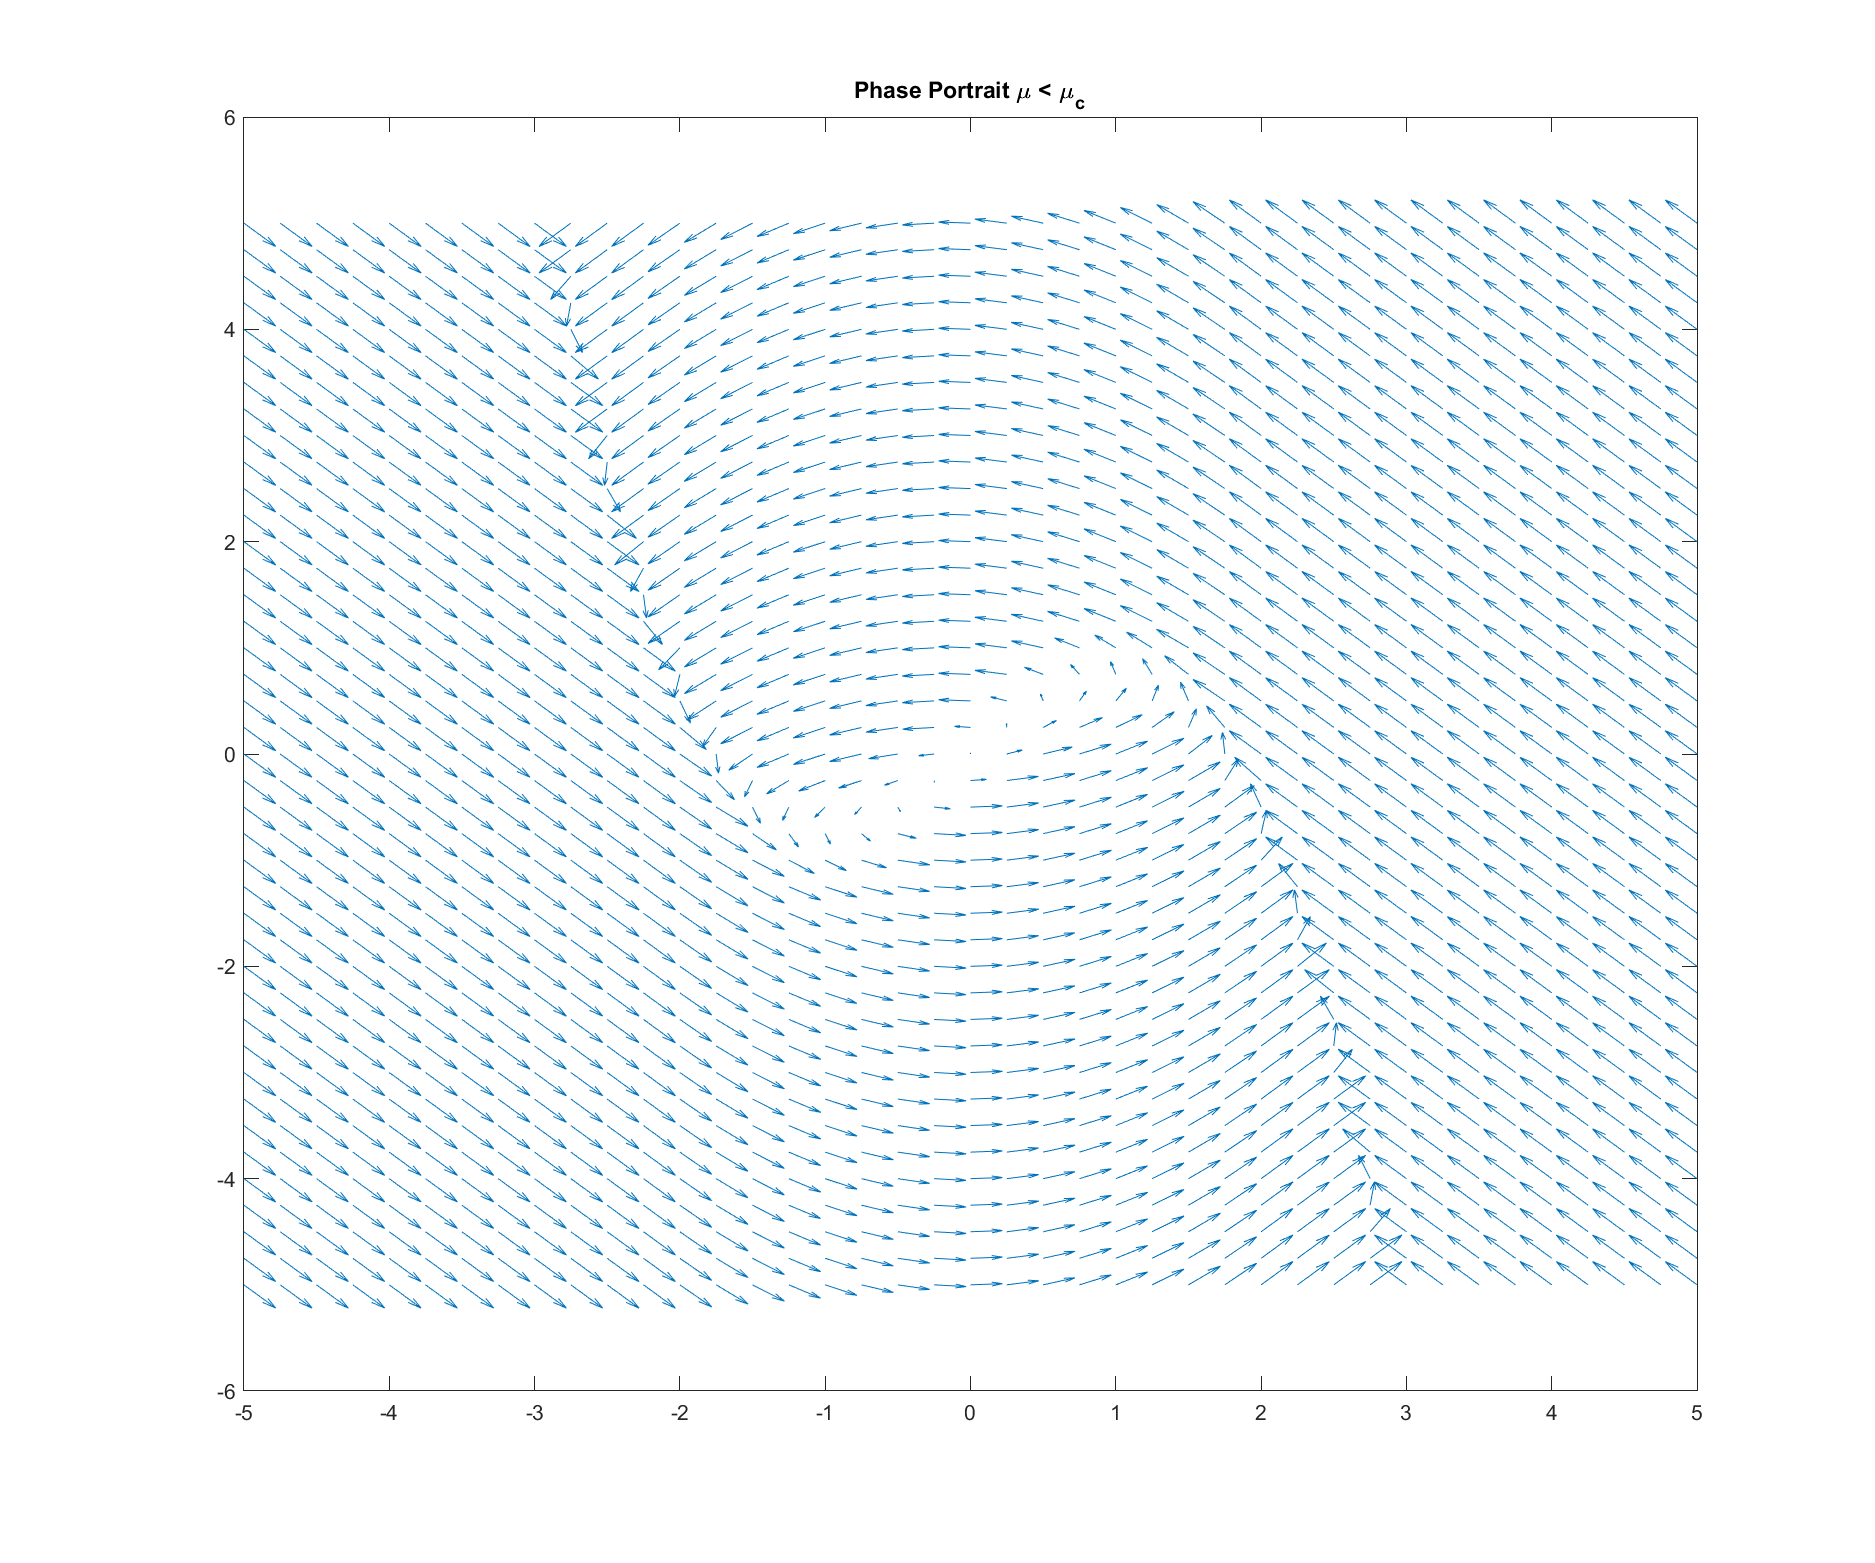
\includegraphics[width=\linewidth]{fig/pblm1_phaseplot_mu01}
	\caption{Phase Portrait for Problem 1 with the parameter below the critical value.}
	\label{fig:pblm1phaseplot_mu01}
\end{figure}


\begin{figure}[p]
	\centering
	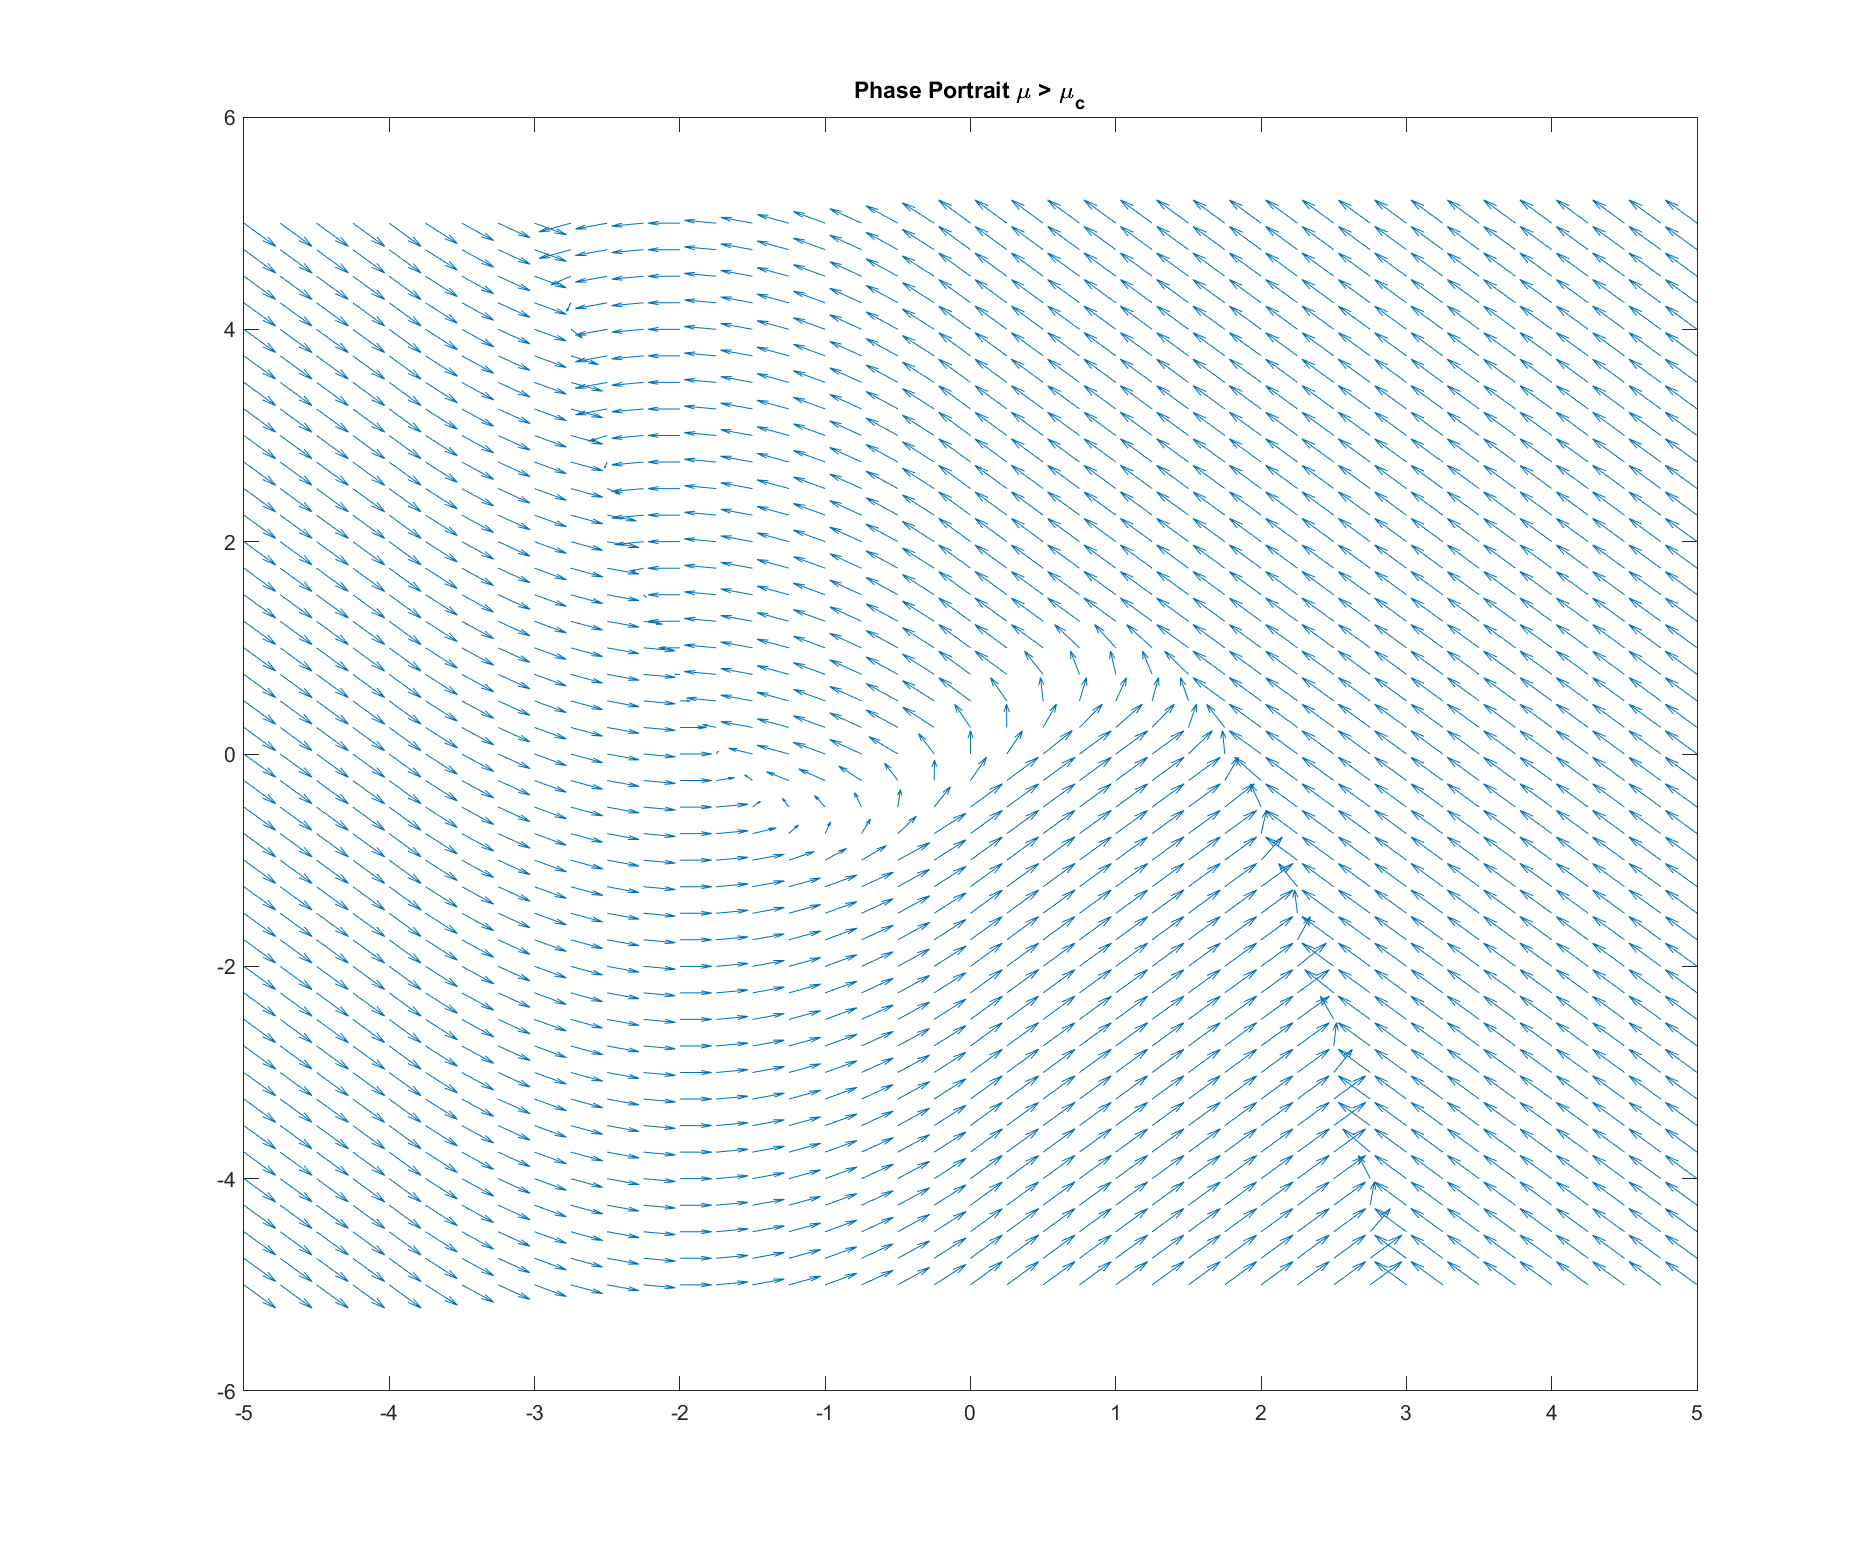
\includegraphics[width=\linewidth]{fig/pblm1_phaseplot_mu2}
	\caption{Phase Portrait for Problem 1 with the parameter above the critical value.}
	\label{fig:pblm1phaseplot_mu2}
\end{figure}

%----------------------------------------------------------------------------
\newpage
\section{Problem 2:}
Consider the system:
\begin{equation}
	\begin{aligned}
		\dot{x}_1 &= -\frac{1}{2} \tan(\frac{\pi x_1}{2}) + x_2\\
		\dot{x}_2 &= x_1 -\frac{1}{2} \tan(\frac{\pi x_2}{2})
	\end{aligned}
\end{equation}


\subsection{Part a}
\textbf{Problem:}
Find all equilibrium points of this system.\\

\noindent
\textbf{Solution:}
The equilibrium points exist whenever $\dot{X} = \mqty[\dot{x}_1\\ \dot{x}_2] = 0$ and can be identified as follows:
\begin{align}
	&\begin{aligned}
		\qty(0) &= -\frac{1}{2} \tan(\frac{\pi x_1}{2}) + x_2\\
		\qty(0) &= x_1 -\frac{1}{2} \tan(\frac{\pi x_2}{2})
	\end{aligned}\\
	\intertext{which becomes:}
	&\begin{aligned}
		x_2 &= \frac{1}{2} \tan(\frac{\pi x_1}{2})\\
		x_1 &= \frac{1}{2} \tan(\frac{\pi x_2}{2})
	\end{aligned}
\end{align}
There are an infinite number of solutions to this set of equations, each of which are equilibrium points.

At each asymptote, there are unstable equilibrium points
\begin{empheq}[innerbox = \fbox]{equation}\label{eq:pblm2a_asm}
	X_{eq} = \mqty[1\\1] + i \mqty[2\\0] + j \mqty[0\\2]
\end{empheq}
with $i = \dots, -1, 0, 1, \dots$ and $j = \dots, -1, 0, 1, \dots$

In addition, any time the each subsequent tangent function intersect with each other another another equilibrium point exists, including, but not exhausted:
\begin{empheq}[innerbox = \fbox]{equation}\label{eq:pblm2a_eqv}
	x = \frac{1}{2} \tan(\frac{\pi x}{2})
	\text{ or }
	x = -\frac{1}{2} \tan(\frac{\pi x}{2})
\end{empheq}

Additionally, within the region around the origin $x \in [-1, 1]$ and $y \in [-1,1]$, 3 distinct equilibrium points exist:
\begin{empheq}[innerbox = \fbox]{equation}\label{eq:pblm2a_origin}
	\begin{aligned}
		X_{eq} &= \mqty[0\\0]\\
		X_{eq} &= \mqty[0.5\\ 0.5]\\
		X_{eq} &= \mqty[-0.5\\ -0.5]
	\end{aligned}
\end{empheq}

\newpage
\subsection{Part b}
\textbf{Problem:}
Use linearization to study the stability of each equilibrium point.\\

\noindent
\textbf{Solution:}
The linearization around individual equilibrium points is given by evaluating the Jacobian matrix which is calculated as:
\begin{align}
	A &= \eval{J_x}_{X = X_{eq}}
	= \eval{\mqty[\dv{f_1}{x_1}&\dv{f_1}{x_2}\\\dv{f_2}{x_1}&\dv{f_2}{x_2}]}_{X=X_{eq}}\\
	&= \eval{\mqty[-\frac{\pi}{4}\qty(\tan[2](\frac{\pi x_1}{2}) + 1)&1\\ 1 &-\frac{\pi}{4}\qty(\tan[2](\frac{\pi x_2}{2}) + 1)]}_{X=X_{eq}}
\end{align}

Using the nlsys class I developed in MATLAB, see \appendixname \ \ref{apx:matlab}, multiple Equilibrium points were linearized and stability was analyzed.

It was determined based on the eigenvalues of the linear systems that all the "equilibrium points" occurring at asymtopes \eqref{eq:pblm2a_asm} were all unstable, the asymptopes (that were checked) satisfying \eqref{eq:pblm2a_eqv} were asymptotically stable, and the analysis of the 3 important equilibrium points \eqref{eq:pblm2a_origin} are addressed below:

The origin itself was determined to be unstable given the dynamics matrix and eigenvalues:
\begin{empheq}[innerbox = \fbox]{equation}\label{eq:pblm2b_origin}
	\begin{aligned}
		&X_{eq} = \mqty[0\\ 0]
		&A = \mqty[-0.7854 & 1\\ 1 & -0.7854]
		&&\begin{aligned}
			\lambda_{1} &= -1.7854\\
			\lambda_{2} &= \ \ 0.2146
		\end{aligned}
	\end{aligned}
\end{empheq}

The quadrant 1 and 3 systems were determined to be asymptotically stable given the dynamics matrix and eigenvalues:
\begin{empheq}[innerbox = \fbox]{equation}\label{eq:pblm2b_quad1}
	\begin{aligned}
		&X_{eq} = \mqty[0.5\\ 0.5]
		&A = \mqty[-1.5708 & 1\\ 1 & -1.5708]
		&&\begin{aligned}
			\lambda_{1} &= -2.5708\\
			\lambda_{2} &= -0.5708
		\end{aligned}
	\end{aligned}
\end{empheq}
\begin{empheq}[innerbox = \fbox]{equation}\label{eq:pblm2b_quad3}
	\begin{aligned}
		&X_{eq} = \mqty[-0.5\\ -0.5]
		&A = \mqty[-1.5708 & 1\\ 1 & -1.5708]
		&&\begin{aligned}
			\lambda_{1} &= -2.5708\\
			\lambda_{2} &= -0.5708
		\end{aligned}
	\end{aligned}
\end{empheq}

\newpage
\subsection{Part c}
\textbf{Problem:}
Using quadratic Lyapunov functions, estimate the region of attraction of each asymptotically stable equilibrium point.
% Try to make your estimates as large as possible
\\

\noindent
\textbf{Solution:}
%Let,
%\begin{equation}
%	V(x) = \frac{1}{2} x_1^2 + \frac{1}{2} x_2^2
%\end{equation}
%
%\begin{align}
%	\dot{V}(x) &= x_1 \dot{x}_1 + x_2 \dot{x_2}\\
%	&= x_1 (-\frac{1}{2} \tan(\frac{\pi x_1}{2}) + x_2) + x_2 (x_1 -\frac{1}{2} \tan(\frac{\pi x_2}{2}))\\
%	&= -\frac{1}{2}\qty(x_1 \tan(\frac{\pi x_1}{2}) + x_2 \tan(\frac{\pi x_2}{2})) + 2 x_1 x_2
%\end{align}


For the asymptotically stable equalibrium point in quadrant 1, a relative system can be defined with $$\tilde{x} = x-x_{eq}$$ resulting in
\begin{align}
	f(\tilde{x}) 
	&= \mqty[-\frac{1}{2} \tan(\frac{\pi (\tilde{x}_1 + x_{1eq})}{2}) + \tilde{x}_2 + x_{2eq}\\ -\frac{1}{2} \tan(\frac{\pi (\tilde{x}_2 + x_{2eq})}{2}) + \tilde{x}_1 + x_{1eq}]\\
	&= \mqty[-\frac{1}{2} \tan(\frac{\pi \tilde{x}_1}{2} + \frac{\pi}{4}) + \tilde{x}_2 + \frac{1}{2}\\ -\frac{1}{2} \tan(\frac{\pi \tilde{x}_2}{2} + \frac{\pi}{4}) + \tilde{x}_1 + \frac{1}{2}]
\end{align}
Additionally, an invarient set boundary can be defined by $$\tilde{x}_1^2 + \tilde{x}_2^2 = r^2$$ which represents a simple radial boundary.\\
The maximum positive invariant set boundary can be calculated by solving for $r$ s.t. $$f^T(x) \cdot \grad{V(x)} \leq 0$$ and is shown as follows:
\begin{align}
	V(x) &= \tilde{x}_1^2 + \tilde{x}_2^2 = r^2\\
	\grad{V(x)} &= \mqty[2 \tilde{x}_1\\ 2 \tilde{x}_2]\\
	f^T(x) \cdot \grad{V(x)} &= \mqty[-\frac{1}{2} \tan(\frac{\pi \tilde{x}_1}{2} + \frac{\pi}{4}) + \tilde{x}_2 + \frac{1}{2}\\ -\frac{1}{2} \tan(\frac{\pi \tilde{x}_2}{2} + \frac{\pi}{4}) + \tilde{x}_1 + \frac{1}{2}]^T \mqty[2 \tilde{x}_1\\ 2 \tilde{x}_2]\\
	&\begin{aligned}
		=&\qty(-\frac{1}{2} \tan(\frac{\pi \tilde{x}_1}{2} + \frac{\pi}{4}) + \tilde{x}_2 + \frac{1}{2})(2\tilde{x}_1)\\
		&+\qty(-\frac{1}{2} \tan(\frac{\pi \tilde{x}_2}{2} + \frac{\pi}{4}) + \tilde{x}_1 + \frac{1}{2})(2\tilde{x}_2)
	\end{aligned}\\
	&\begin{aligned}
		=& \ \tilde{x}_1\tan(\frac{\pi \tilde{x}_1}{2} + \frac{\pi}{4}) + \tilde{x}_2 \tan(\frac{\pi \tilde{x}_2}{2} + \frac{\pi}{4})\\
		&+4\tilde{x}_1 \tilde{x}_2 + \tilde{x}_1 +\tilde{x}_2
	\end{aligned}
\end{align}
Which when solved results in a conservative region of attraction of radius $r\leq0.5$. (or maybe strictly less-than... calculator acted funny when solving it)

Additionally, when the process was repeated for the 3rd quadrant equilibrium point, the results were the same and the conservative region of attraction had a radius of $r=0.5$.

A few other equilibrium points were tested and it was clear that the asymptotic eq-points were unstable, but of the other stable eq-points (done numerically) they were all very very conservative results using this method. (SOS is probably a better option... or perhaps a more complicated elliptical bound instead)

\newpage
\subsubsection{Part d}
\textbf{Problem:}
Plot the phase portrait of the system and show on it the exact regions of attraction as well as your estimates.\\

\noindent
\textbf{Solution:}
The phase portrait of the system was plotted along with the important indicators for equilibrium points and boundary regions as seen in \figurename \ \ref{fig:pblm2phaseplot}, \figurename \ \ref{fig:pblm2phaseplot_zoomOut}, and \figurename \ \ref{fig:pblm2phaseplot_origin}.


\begin{figure}[h]
	\centering
	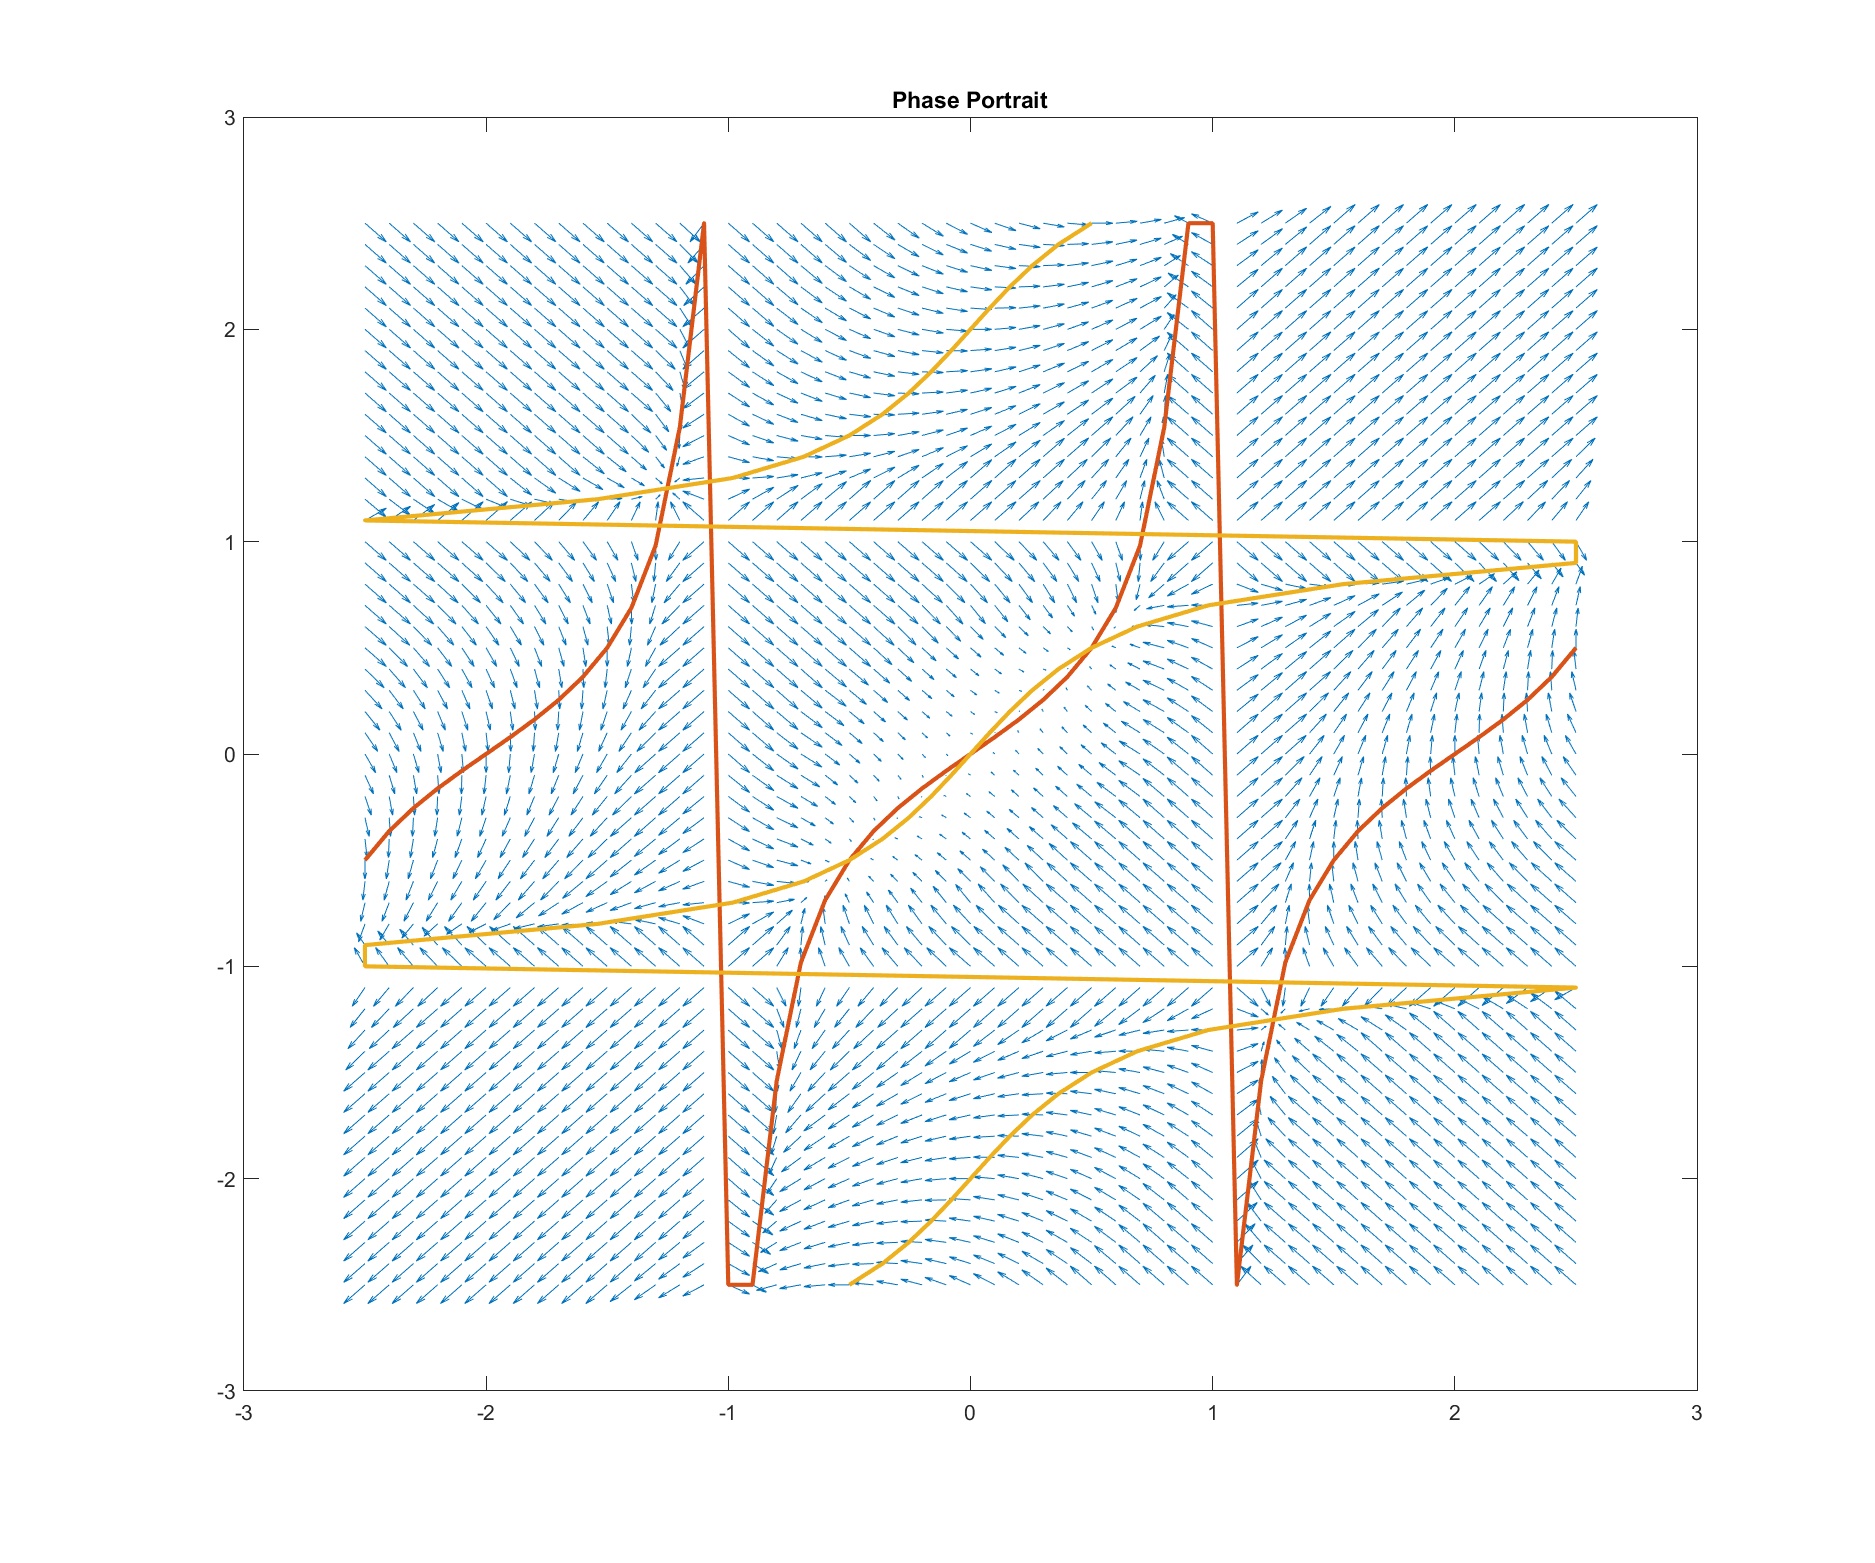
\includegraphics[width=\linewidth]{fig/pblm2_phaseplot}
	\caption{Phase Portrait for Problem 2}
	\label{fig:pblm2phaseplot}
\end{figure}

\begin{figure}[p]
	\centering
	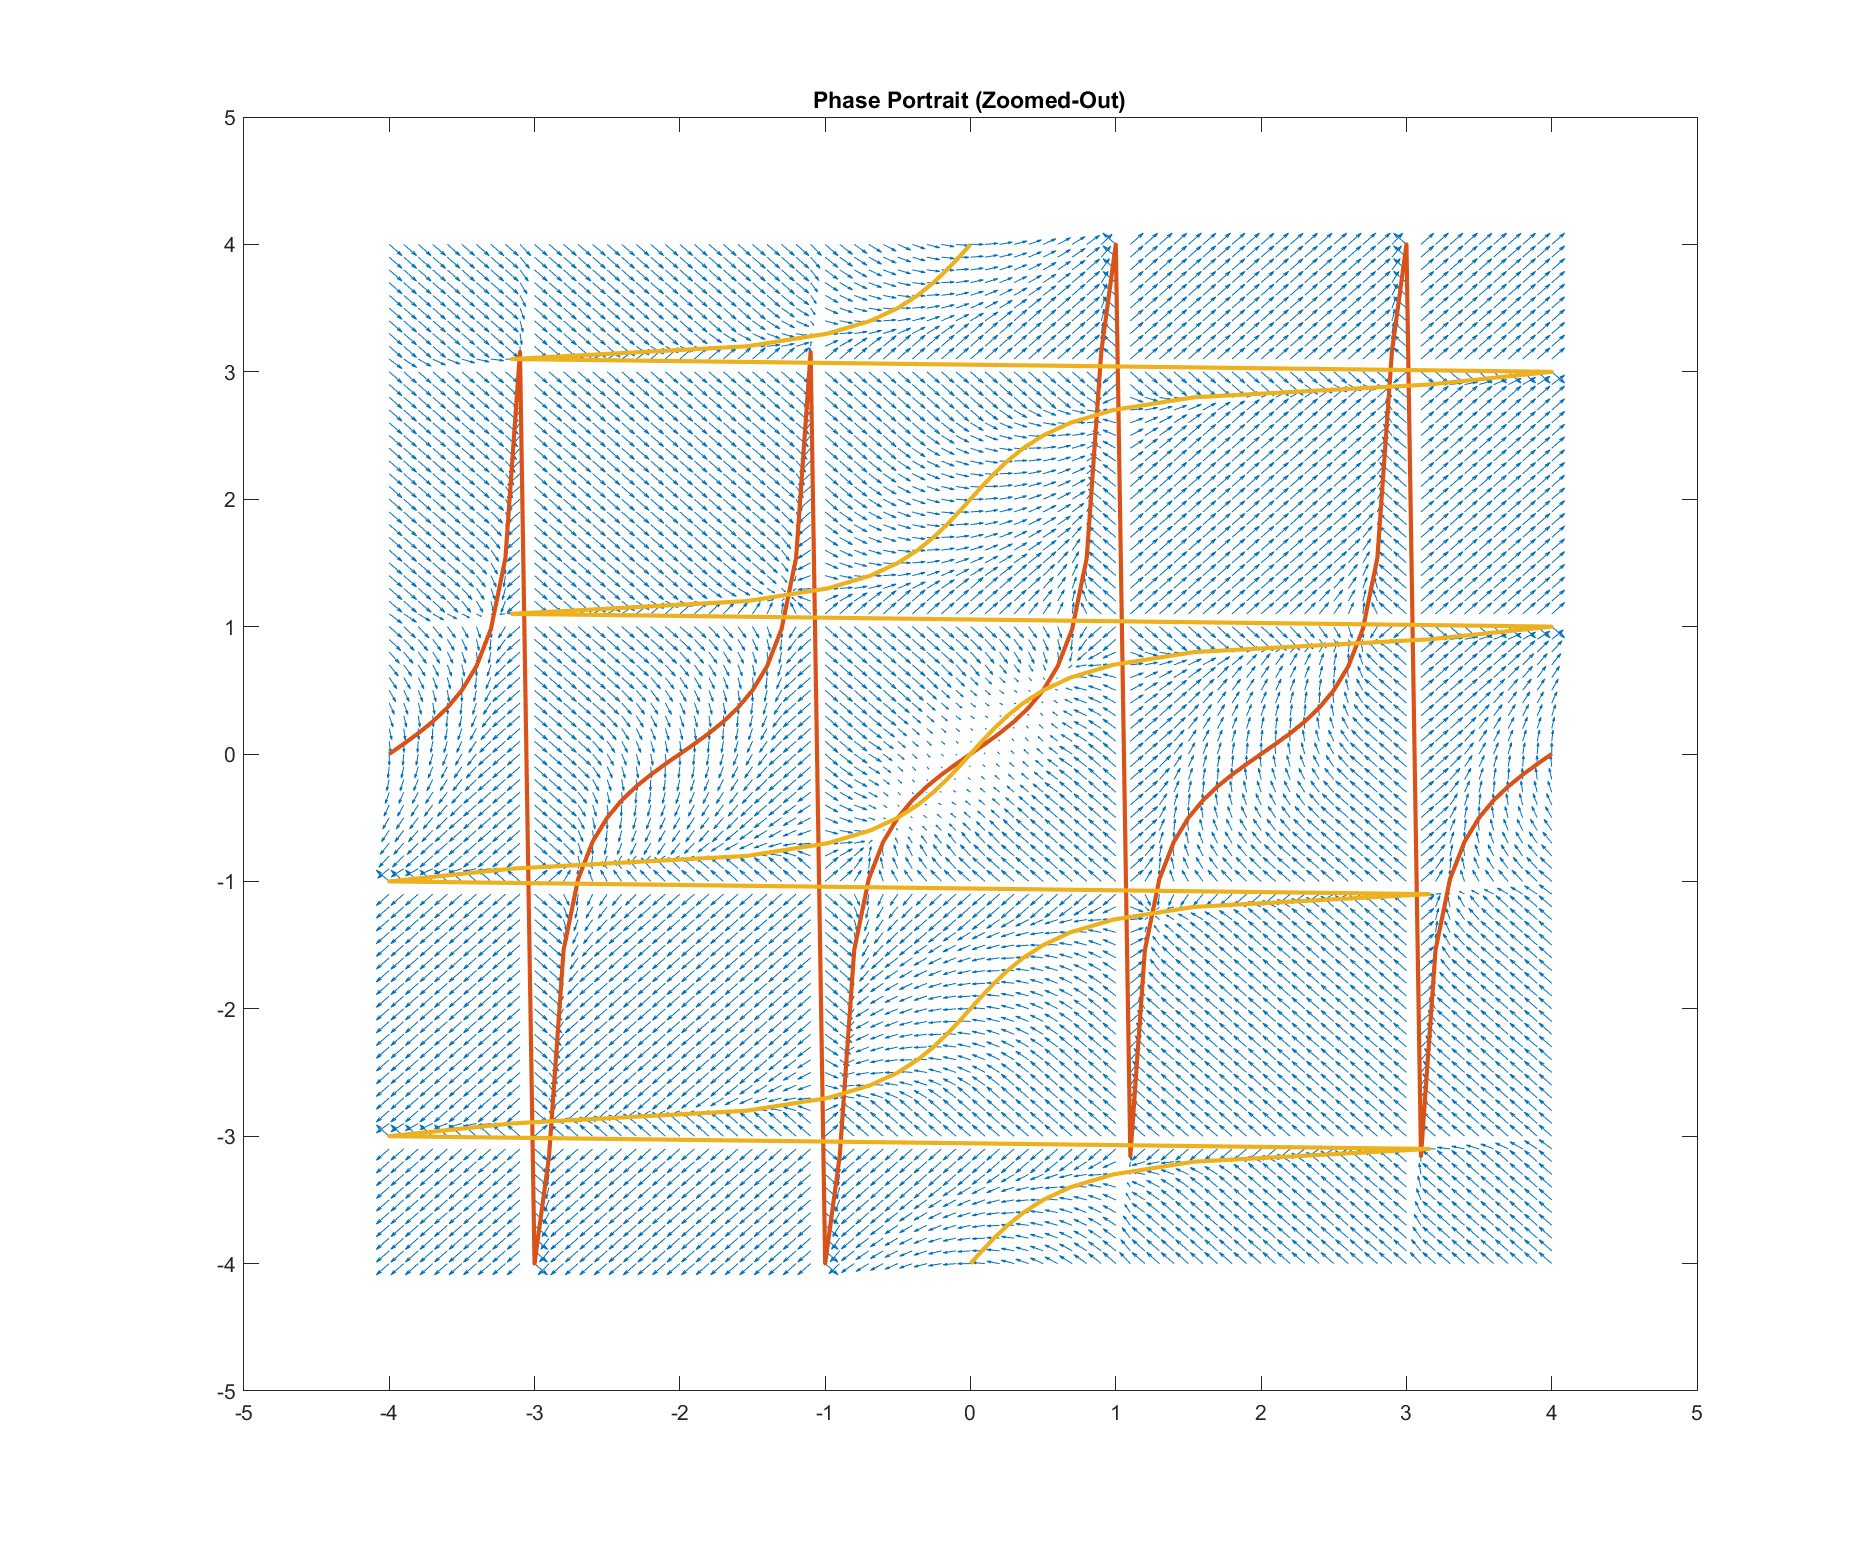
\includegraphics[width=\linewidth]{fig/pblm2_phaseplot_zoomOut}
	\caption{Phase Portrait for Problem 2 that is zoomed out to demonstrate the infinite nature of equilibrium points.}
	\label{fig:pblm2phaseplot_zoomOut}
\end{figure}


\begin{figure}[p]
	\centering
	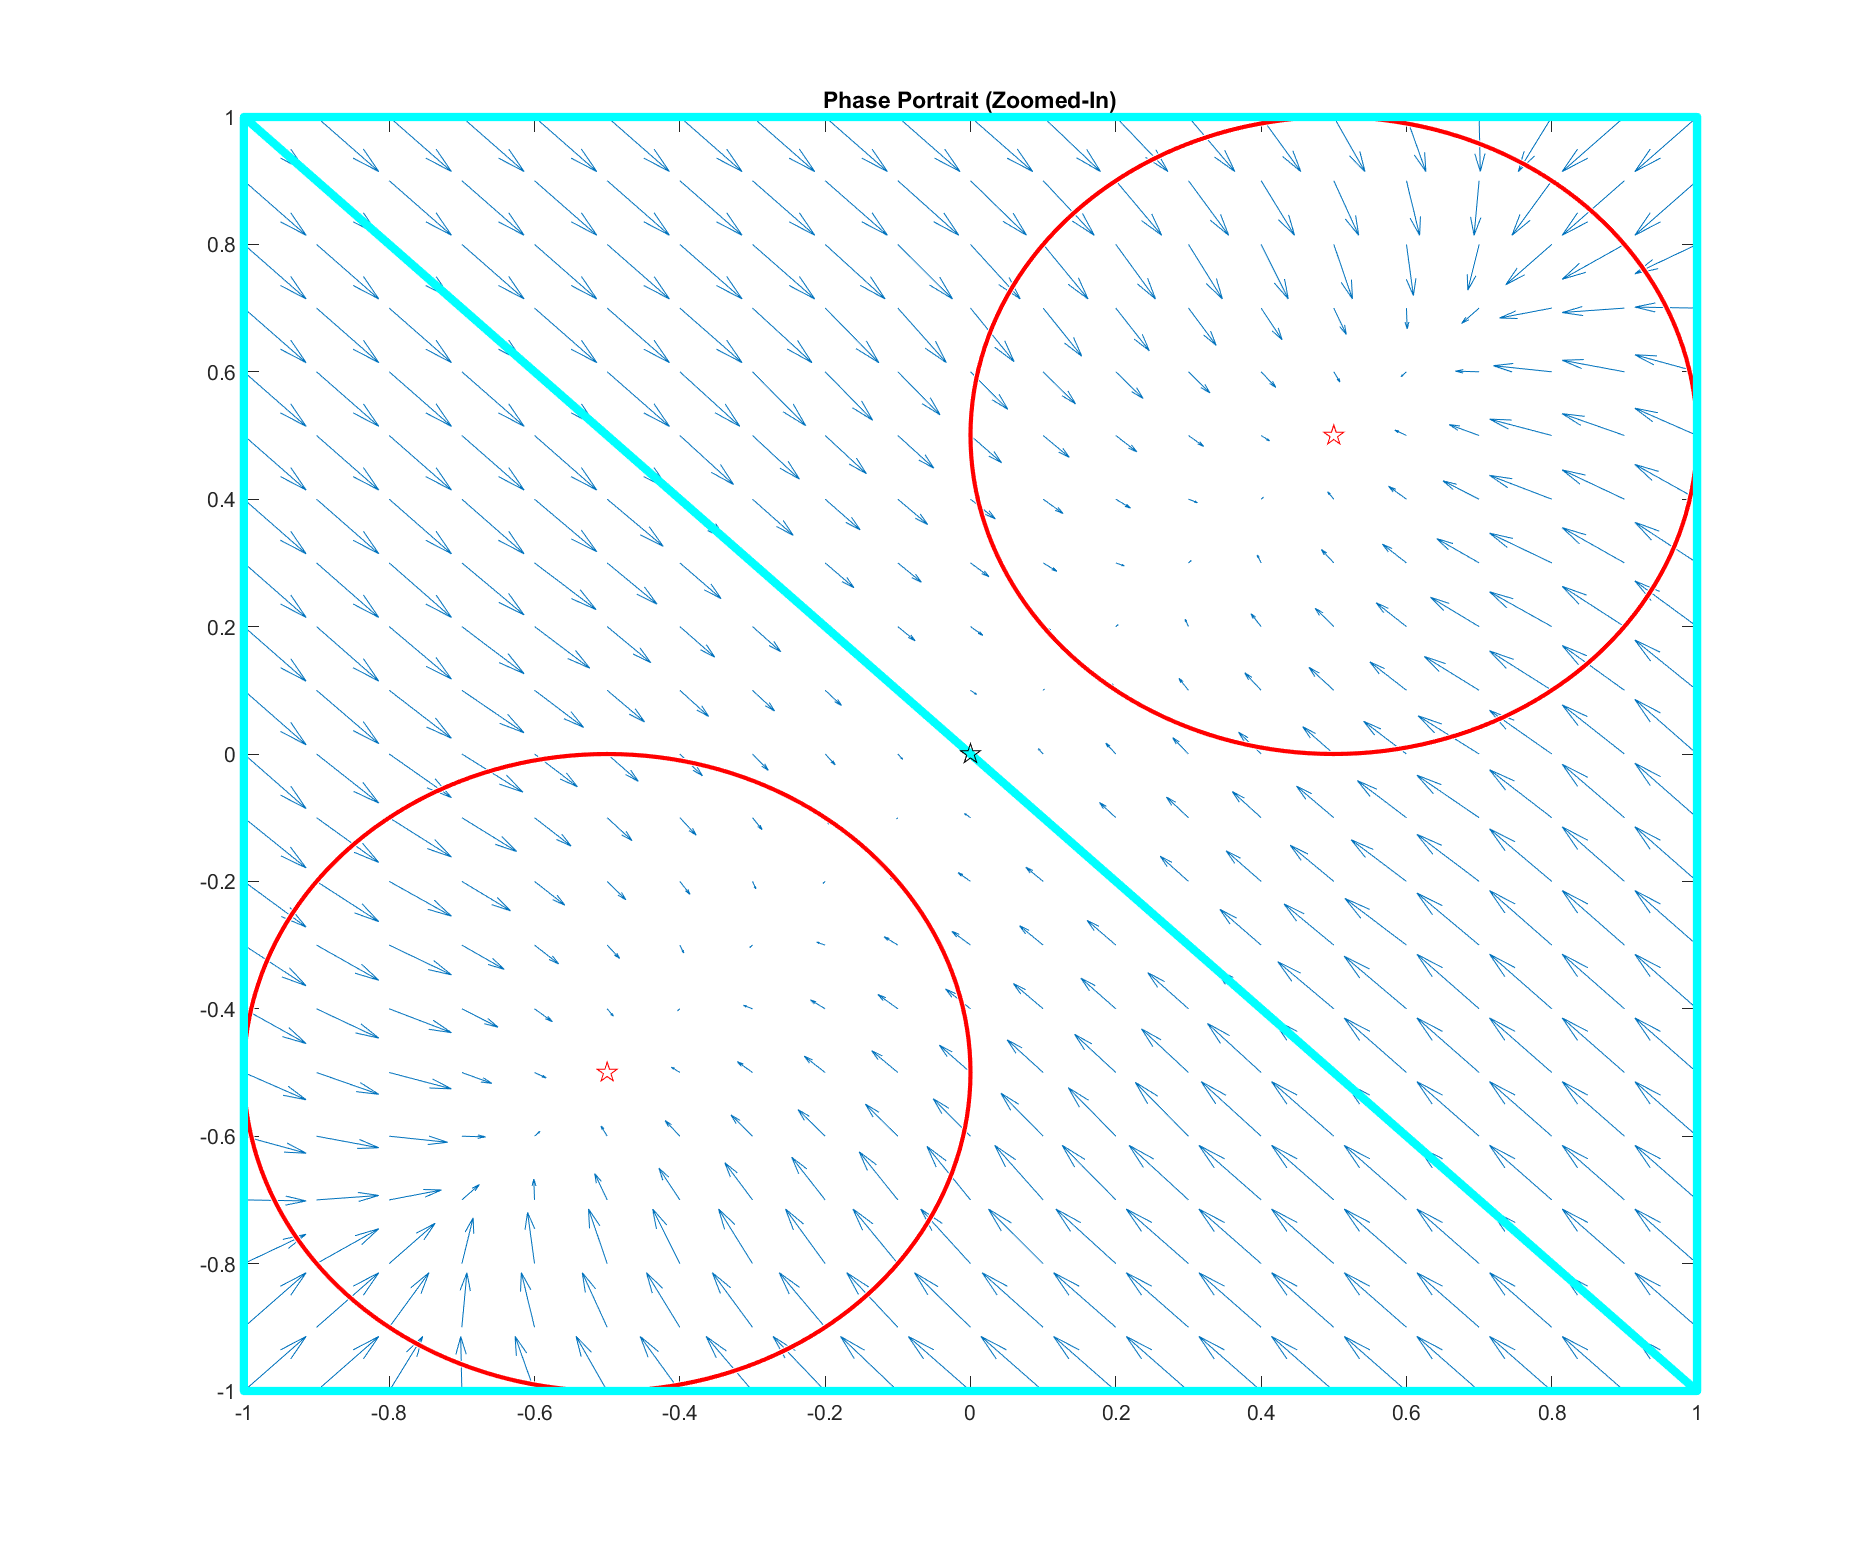
\includegraphics[width=\linewidth]{fig/pblm2_phaseplot_origin}
	\caption{Phase Portrait for Problem 2 focusing on the origin with regions of convergences and equilibrium points.}
	\label{fig:pblm2phaseplot_origin}
\end{figure}

%----------------------------------------------------------------------------
\newpage
\section{Problem 3}
\textbf{Problem:}
Prove that the origin is the globally asymptotically stable equilibrium point of the system
\begin{equation}
	\begin{aligned}
		\dot{x}_1 &= -x_1 - \sat(x_3)\\
		\dot{x}_1 &= -x_2 - \sat(x_1)\\
		\dot{x}_1 &= -x_3 - \sat(x_2)
	\end{aligned}
\end{equation}
where
\begin{equation}
	\sat(x) := \sign(x) \min\{1,\abs{x}\}
\end{equation}

\noindent
\textbf{Solution:}
% this is one of the feedback problems like in the last hmk
\subsection{System and Storage Function Definition}
This system can be rewritten in a coupling feedback system $H$ and $K$ defined as:
\begin{align}
	H &= \mqty[\dmat{H_1}{H_2}{H_3}], \hspace{0.25in}
	H_i
	=\begin{cases}
		\dot{x}_i = f(x_i) + g(x_i) u_i\\
		y_i = h(x_i)
	\end{cases}\\
	K &= \mqty[	 0 	& 0 &-1\\
	-1 	& 0 & 0\\
	0 	&-1 & 0]
\end{align}
where $K$ is the coupling matrix of the individual nonlinear subsystems with the following specific definitions:
\begin{equation}
	H_i =
	\begin{cases}
		\dot{x}_i = -x_i + u_i\\
		y_i = h_i(x_i)
	\end{cases}
\end{equation}
where $h_i(x_i) = \sat(x_i)$.

A storage function for each of the individual subsystems can be defined as:
\begin{equation}
	V_i(x_i) = \int_{0}^{x_i} h_i(\eta) \dd \eta
\end{equation}

Taking a look at the change of the storage function over time, the output strict passivity can be proven by:
\begin{align}
	\dot{V}_i (x_i) &= \dv{V_i}{x_i} \dot{x}_i\\
	&= \dv{x_i} \int_0^{x_i} h_i(\eta) \dd{\eta} \dot{x}_i\\
	&= h_i(x_i) \dot{x}_i
	\intertext{taking the definition for $\dot{x}_i$ and relating $h_i(x_i) = y_i$,}
	&= h_i(x_i) (-x_i + u_i)\\
	&= -x_i h_i(x_i) + u_i y_i
\end{align}

\newpage
\subsection{Probing Input/Output Passivity}
In order to guarantee Input passivity, the system must satisfy the following inequality:
\begin{align}
	x h(x) &\leq \delta_i x^2\\
	x (\sat(x)) &\leq \delta x^2
\end{align}
by definition, $\sat(x) := \sign(x) \min\{1,\abs{x}\}$, thus the following inequalities apply:
\begin{align}
	\begin{cases}
		\sat(x) > 0, &x>0\\
		\sat(x) < 0, &x<0
	\end{cases}
\end{align}
therefore, the input passivity equality holds.

Since the input passivity holds, a $\delta_i$ will exist s.t.,
\begin{align}
	x_i h_i(x_i) &\leq \delta_i x^2\\
	x_i (h_i(x_i) - \delta_i x_i) &\leq 0
\end{align}
clearly, $x_i h_i(x_i)$ can then be bounded from below by: % since \abs{h_i} \leq \abs{\delta_i x} \forall x
\begin{align}
	x_i h_i (x) \geq \frac{1}{\delta_i} h_i^2(x_i)\\
	-x_i h_i (x) \geq -\frac{1}{\delta_i} h_i^2(x_i)\\
	\intertext{since $y_i = h_i(x_i)$,}
	-x_i h_i (x) \geq -\frac{1}{\delta_i} y_i^2(x_i)
\end{align}\\

Therefore, this demonstrates Output Strict Passivity:
\begin{align}
	\dot{V}_i &\leq -\frac{1}{\delta_i} y_i^2 + y_i u_i\\
	\intertext{or with $d_i = \frac{1}{\delta_i}$ and }
	\dot{V}_i &\leq d_i y_i^2 + y_i u_i
\end{align}
and the passivity theorem can then be applied.\\

\newpage
\subsection{Applying Passivity Theorem}
Let $$\epsilon_i = \frac{1}{\delta_i}$$ and then define
\begin{align}
	A &= - \text{diag}\{\epsilon_i\} + K\\
	P &= \text{diag}\{d_i\}
\end{align}
which for this $3^{rd}$-order system can be written as
\begin{align}
	A &= -\mqty[\dmat{\epsilon_1}{\epsilon_2}{\epsilon_3}] + \mqty[0 & 0 &-1\\ -1 & 0 & 0\\ 0 &-1 & 0] 
	= \mqty[-\epsilon_1 & 0 &-1\\
	-1 &-\epsilon_2 &0\\
	0	&-1	&-\epsilon_3]\\
	P &= \mqty[\dmat{d_1}{d_2}{d_3}]
\end{align}

Appropriate values for A and P can be found to prove stability of the full feedback interconnection using the following inequality:
\begin{align}
	A^T P + P A &\leq 0
\end{align}

This can then be further developed to prove Global Asymptotic Stability by making it a strict inequality like so:
\begin{align}
	A^T P + P A &< 0
\end{align}

This can be written with the actual matrices as
\begin{align}
	\mqty[-\epsilon_1 & 0 &-1\\
	-1 &-\epsilon_2 &0\\
	0	&-1	&-\epsilon_3]^T
	\mqty[\dmat{d_1}{d_2}{d_3}] +
	\mqty[\dmat{d_1}{d_2}{d_3}]
	\mqty[-\epsilon_1 & 0 &-1\\
	-1 &-\epsilon_2 &0\\
	0	&-1	&-\epsilon_3]
	&< 0
\end{align}

\begin{align}
	\mqty[-d_1\epsilon_1 & -d_1 &0\\
	0 &-d_2\epsilon_2 &-d_2\\
	-d_3	&0	&-d_3\epsilon_3]+
	\mqty[-d_2\epsilon_1 & 0 &-d_1\\
	-d_2 &-d_2\epsilon_2 &0\\
	0	&-d_3	&-d_3\epsilon_3]
	&< 0
\end{align}

\begin{align}
	\mqty[-2 d_1\epsilon_1 & -d_1 &-d_1\\
	-d_2 &-2 d_2\epsilon_2 &-d_2\\
	-d_3	&-d_3	&-2 d_3\epsilon_3]
	&< 0
\end{align}
or equivalently
\begin{align}
	\mqty[2 d_1\epsilon_1 & d_1 &d_1\\
	d_2 &2 d_2\epsilon_2 &d_2\\
	d_3	&d_3	&2 d_3\epsilon_3]
	&> 0
\end{align}

\newpage
The positive definiteness can be determined by
\begin{align}
	2 d_1 \epsilon_1 &>0\\
	\mqty|2 d_1\epsilon_1 & d_1\\
	d_2 &2 d_2\epsilon_2| = d_1 d_2 (4 \epsilon_1 \epsilon_2 - 1) &> 0\\
	\mqty|2 d_1\epsilon_1 & d_1 &d_1\\
	d_2 &2 d_2\epsilon_2 &d_2\\
	d_3	&d_3	&2 d_3\epsilon_3|
	= d_1 d_2 d_3  (8 \epsilon_1 \epsilon_2 \epsilon_3 - 2 \epsilon_1)\nonumber\\
	- d_1 d_2 d_3(2 \epsilon_3 - 1)
	+ d_1 d_2 d_3 (1 - 2\epsilon_2)\nonumber\\
	= d_1 d_2 d_3 (8 \epsilon_1 \epsilon_2 \epsilon_3 
	- 2 \epsilon_1
	- 2 \epsilon_2
	- 2 \epsilon_3)
	&>0
\end{align}
From this and the definition of $d_i > 0$, these inequalities can be equated to
\begin{align}
	\epsilon_1&>0\\
	4 \epsilon_1 \epsilon_2 -1 &>0\\
	4 \epsilon_1 \epsilon_2 \epsilon_3 - \epsilon_1 - \epsilon_2 - \epsilon_3 &> 0	
\end{align}
Returning to the original definition of $\epsilon_i = \frac{1}{\delta_i}$ and the limitation of $x \sat(x) \leq \delta_i x^2$,
it can be seen that a selection of $\delta_i = 1 \ \forall i=1,2,3$ is valid and thus $$\epsilon_1 = \epsilon_2 = \epsilon_3 = 1$$
which can be used to satisfy the inequalities:
\begin{align}
	(1) = 1&>0\\
	4 (1) (1) -1 = 3 &>0\\
	4 (1) (1) (1) - (1) - (1) - (1) = 1 &> 0	
\end{align}

Therefore, it can be seen said that the origin for the coupled feedback system is Globally Asymptotically Stable.


%----------------------------------------------------------------------------
\newpage
\section{Problem 4}
\textbf{Problem:}
Comment on the existence/uniqueness of solutions for the systems below. Provide
your reasons.\\

\subsection{Part a}
\begin{equation}
	\dot{x} = x^2
\end{equation}
\noindent
\textbf{Solution:}
Assuming that the system is defined for $x\in \real$, existence and uniqueness can be guaranteed by ensuring certain continuity conditions exist.\\
Since the function $f(x) = x^2$ is a continuous function $\forall x \in \real$, it can be said that a solution does exist.\\
Additionally, since $f(x)$ is locally Lipschitz continuous, i.e. $\dv{f}{x} = 2 x$ is continuous, it can be said that a unique solution exists for $t \in [0,t_f)$.\\
However, $f(x)$ is not globally Lipschitz continous, since $\norm{\dv{f}{x}} = \norm{2x} \nleq L \forall x \in \real^n$, (which can be more rigorously proven as this was only a sufficient condition) the uniqueness of a solution cannot be garunteed for $t \in [0,\infty)$.

\subsection{Part b}
\begin{equation}
	\dot{x} = \sqrt{x}
\end{equation}
\noindent
\textbf{Solution:}
Assuming that the system is defined for $x \geq 0$, existence and uniqueness can be guaranteed by ensuring certain continuity conditions exist.\\
Since the function $f(x) = x^2$ is a continuous function $\forall x \geq 0$, it can be said that a solution does exist.\\
However, a unique solution cannot be guaranteed as the function is not Liptchitz continuous directly around $x=0$ as the slope becomes infinite and cannot be bounded by a Liptchitz constant.

\subsection{Part c}
\begin{equation}
	\dot{x} = 1 + \cfrac{1 + x^3}{1 + x^4}
\end{equation}
\noindent
\textbf{Solution:}
Assuming that the system is defined for $x\in \real$, existence and uniqueness can be guaranteed by ensuring certain continuity conditions exist.\\
Since the function $f(x)$ is a continuous function $\forall x \in \real$, it can be said that a solution does exist.\\
Additionally, the system is also continuously differentiable:
$$\dv{f}{x} = \dv{x} \qty(1 + \cfrac{1 + x^3}{1 + x^4}) = \frac{-x^2(x^4 - 2x - 3)}{(1+x^4)^2}$$
and its derivative is bounded
$$\norm{\frac{-x^2(x^4 - 2x - 3)}{(1+x^4)^2}} \leq L$$
by the positive constant $L < \infty$. This implys that the system is globally Lipshitz continuous and therefore a unique solution is guaranteed to exists for $t \in [0,\infty)$.

%----------------------------------------------------------------------------
\newpage
\section{Problem 5}
\textbf{Problem:}
Show that the following system contains no closed orbits.
\begin{equation}
	\begin{aligned}
		\dot{x}_1 &= -x_1 + x_2^3 + 1\\
		\dot{x}_2 &= -4x_1^2 + 3 x_2
	\end{aligned}
\end{equation}

\noindent
\textbf{Solution:}
Sufficient conditions to proving that no closed orbits exist are that
If $\div{f} \neq 0 \forall x \in D$ and does not change sign within a simply connected region $D$.
Let $D = x\in\real^2$. The divergence is given as:
\begin{align}
	\div{f} &= \dv{f_1}{x_1} + \dv{f_2}{x_2}\\
	&= -1 + 3\\
	&= 4
\end{align}
Since $\div{f}$ is constant (and not identically zero) within the entire region $D$, there is sufficient evidence to say that no periodic orbits exist and therefore the system has no closed orbits.


%----------------------------------------------------------------------------
\newpage
\section{Problem 6}
\textbf{Problem:}
Prove that the origin is the globally asymptotically stable equilibrium of the following system.
\begin{equation}
	\begin{aligned}
		\dot{x}_1 &= x_2\\
		\dot{x}_2 &= -(\sin(x_1) + 2)(x_1 + x_2)
	\end{aligned}
\end{equation}

\noindent
\textbf{Solution:}
\subsection{Initial Linearized System Stability}
The linearization around individual equilibrium points is given by evaluating the Jacobian matrix which is calculated as:
\begin{align}
	A &= \eval{J_x}_{X = X_{eq}}
	= \eval{\mqty[\dv{f_1}{x_1}&\dv{f_1}{x_2}\\\dv{f_2}{x_1}&\dv{f_2}{x_2}]}_{X=X_{eq}}\\
	&= \eval{\mqty[0 & 1\\
		-(\sin(x_1) + x_1 \cos(x_1) + 2 + x_2 \cos(x_1)) & -(\sin(x_1) + 2)
		]}_{x_1 = x_2 = 0}\\
	&= \mqty[0&1\\-2 &-2]
\end{align}

The dynamics of this linearized system are described by the characteristic polynomial calculated as:
\begin{align}
	\Delta(s) = \det(sI - A)
	&= \det\mqty[s &-1\\ 2 &s+2]\\
	&= s(s+2) - (-1) (2)\\
	\Aboxed{\Delta(s) &= s^2 + 2s + 2}
\end{align}

The roots of this polynomial are then calculated as the eigenvalues:
\begin{align}
	\Aboxed{\lambda_{1,2} &= -1 \pm j 1}
\end{align}

From this it is apparent that, locally, there exists a stable focus around the origin.

\newpage
\subsection{Lyapnov Method}
The maximum positive invariant set boundary can be calculated by solving for $r$ s.t. $$f^T(x) \cdot \grad{V(x)} \leq 0$$ and is shown as follows:
\begin{align}
	V(x) &= x_1^2 + x_2^2 = r^2\\
	\grad{V(x)} &= \mqty[2 x_1\\ 2 x_2]\\
	f^T(x) \cdot \grad{V(x)}
	&= \mqty[x_2 &-(\sin(x_1) + 2)(x_1 + x_2)] \mqty[2 x_1\\ 2 x_2]\\
	&= 2 x_1 x_2 - 2 x_2(x_1 \sin(x_1) + 2 x_1 + x_2 \sin(x_1) + 2 x_2)\\
	&= 2 x_1 x_2 - 2 x_1 x_2 \sin(x_1) - 4 x_1 x_2 - 2 x_2^2 \sin(x_1) - 4 x_2^2\\
	&= -2 x_1 x_2 (1 + \sin(x_1)) - 2 x_2^2 (2 + \sin(x_1))
\end{align}
The second term is clearly not problimatic: $$- 2 x_2^2 (2 + \sin(x_1)) \leq 0, \ \forall x_1,x_2 \in \real$$

However, the first term is not as straight forward. It is true that $$1+\sin(x_1) \geq 0$$ and that in quadrants 1 and 3, the term satisfies the requirements. In quadrants 2 and 4 it becomes problematic as the term does not always remain negative. However, it is possible to prove that the boundary region itself is unbounded as $$\abs{2x_1 x_2(1+sin(x_1))} \leq \abs{2x_2^2 (2+sin(x_1))}, \forall \ x_1,x_2 \in \real$$
This leads to the conclusion that the system is Globally Asymptotically Stable since the region of convergence is $x_1,x_2 \in \real$.










\newpage
\appendix
\section{MATLAB Code:}\label{apx:matlab}
All code I write in this course can be found on my GitHub repository:\\
\href{https://github.com/jonaswagner2826/MECH6313}{https://github.com/jonaswagner2826/MECH6313}
% MECH6313_HW6
\lstinputlisting[caption={MECH6313\_Exam},label={script:Exam}]{MECH6313_Exam.m}


\end{document}
